\documentclass[11pt]{article}

\usepackage[margin=1in]{geometry}
\usepackage{graphicx}
\usepackage{booktabs}
\usepackage{amsmath}
\usepackage[round]{natbib}
\usepackage[colorlinks=true,linkcolor=blue,citecolor=blue,urlcolor=blue]{hyperref}
\usepackage{xcolor}
\usepackage{caption}
\usepackage{authblk}
\usepackage{enumitem}

\setlength{\parskip}{0.5\baselineskip}
\setlength{\parindent}{0pt}

\title{\textbf{Reliable Machine Learning Under Distribution Shift:\\
Uncertainty-Aware Diabetes Risk Prediction from National Health Survey Data}}

% To add a co-author later: duplicate the \author{} and \affil{} lines below,
% e.g. \author[2]{Co-Author Name} and \affil[2]{Their Affiliation}.
\author[1]{Edmund Eric Gah\thanks{Corresponding author: \texttt{edmund.gah@exealabs.org}}}
\affil[1]{Exea Labs}
\date{}

\begin{document}

\maketitle

% --- Exea Labs mark -----------------------------------------------------
% The pasted image supplied for this could not be saved to a file in the
% authoring environment, so the mark is reproduced faithfully as text
% (it is itself a simple bold wordmark, "/E/"). To use the exact source
% image instead, add it to figures/ (e.g. figures/exealabs_logo.png) and
% replace the line below with:
%   
\includegraphics[width=1.6cm]{figures/exealabs_logo.png}
\vspace{-0.5cm}
\begin{center}
  {\Large\bfseries\sffamily /E/}
\end{center}
\vspace{0.3cm}

\begin{abstract}
Machine-learning models evaluated only on held-out data from their own training distribution can look reliable and then fail silently once deployed, as patient populations and data-collection practices drift across time, geography, and demographic groups. This paper investigates whether calibrated probabilities and conformal prediction reliably flag which predictions of a health-risk model are untrustworthy once its input distribution shifts, using diabetes-risk prediction on the CDC's Behavioral Risk Factor Surveillance System (BRFSS) as the application. Using three real, non-synthetic shift settings---a 6-year temporal shift (2017$\to$2023), demographic subgroups within it, and a single-year geographic shift across US Census regions---together with a fourth analysis testing whether a known remedy corrects the coverage loss found in the third, we find that (1) aggregate temporal degradation is mild but statistically real (AUROC drop 0.0081, 95\% CI [0.0057, 0.0103]), and this average conceals a substantially larger fairness gap by age (AUROC 0.836 at ages 18--44 versus 0.750 at 65+, gap 0.085 [0.078, 0.092]); (2) geographic shift, isolated from time, degrades calibration and conformal coverage far more than six years of temporal shift did (conformal coverage 90.0\%$\to$87.3\% for the South versus 90.0\%$\to$89.7\% temporally); (3) the model's own uncertainty remains informative under every shift tested (failure-detection AUROC 0.80--0.82 throughout); and (4) weighted conformal prediction \citep{tibshirani2019conformal} recovers roughly half the coverage lost to geographic shift, though it comes at a small but statistically significant coverage \emph{cost} in a region with no real shift to correct for---reweighting is a targeted remedy, not a free default. All differences above are 95\% bootstrap confidence intervals (300 resamples) that exclude zero. Together these results argue that shift \emph{magnitude}, not merely shift's presence, determines whether uncertainty-aware safeguards hold---and that evaluating only one shift dimension, or only in aggregate, can miss the failure modes that matter most.
\end{abstract}

\section{Introduction}

A model that occasionally makes an incorrect prediction can still be useful in a clinical or public-health setting; a model that is confidently wrong, and unable to recognize that it has left the population it was trained on, is considerably more dangerous. Standard machine-learning evaluation---a single train/test split, an aggregate accuracy number---does not distinguish these two cases. The gap between them is especially consequential in healthcare, where the populations, practices, and even survey instruments a model encounters after deployment routinely differ from those it was trained on.

This paper asks a more specific question than ``how accurate is the model'': when a health-risk prediction model encounters a distribution shift, does its own uncertainty reliably identify which of its predictions are likely wrong, and can that reliability be restored cheaply once it degrades? We study this using diabetes-risk prediction on BRFSS, a large annual US health survey whose multi-year, multi-region structure supports studying \emph{real} distribution shift directly, rather than the synthetic corruptions common in the uncertainty-quantification literature \citep{ovadia2019trust,koh2021wilds}.

Our contribution is empirical rather than methodological: we apply established techniques---post-hoc calibration, split and weighted conformal prediction, standard fairness metrics---rigorously to a real, underexplored setting, rather than proposing new ones. Concretely:

\begin{enumerate}[leftmargin=*]
\item A 6-year temporal shift analysis (2017 train $\to$ 2019/2021/2023 evaluation) shows performance and calibration degrade only mildly on average.
\item A subgroup fairness analysis shows that this average conceals a large age-related gap the aggregate evaluation misses entirely.
\item A geographic shift analysis, isolated from time within a single year, shows geography to be a substantially larger shift than six years of time---large enough to measurably strain the conformal coverage guarantee.
\item A weighted conformal prediction analysis shows that the theoretically-prescribed fix for that strain works, partially---and reveals a small but real cost where no correction was needed.
\item A deep-ensemble and MC-dropout comparison shows the central finding is not an artifact of gradient-boosted trees: a structurally different model family reaches the same discrimination ceiling and produces a comparably informative uncertainty signal.
\end{enumerate}

Every comparison above carries a 95\% bootstrap confidence interval rather than being reported as a bare point estimate (Section~\ref{sec:metrics})---a methodological choice that itself surfaced one correction to an earlier draft of this analysis, detailed in Section~\ref{sec:weighted-conformal}.

\section{Related Work}

Prior work shows that standard classifiers become both less accurate and poorly calibrated under dataset shift, and that common uncertainty estimates---including deep ensembles and MC-dropout---degrade in reliability precisely when they are needed most \citep{ovadia2019trust,lakshminarayanan2017ensembles,gal2016dropout}. Post-hoc calibration methods such as Platt scaling and isotonic regression are effective in-distribution, but their behavior under shift is comparatively under-studied \citep{guo2017calibration,niculescu2005predicting}. Conformal prediction offers distribution-free coverage guarantees under exchangeability \citep{vovk2005algorithmic}, but these guarantees provably degrade under covariate shift, which has motivated weighted and adaptive variants \citep{tibshirani2019conformal}---the method we apply directly in Section~\ref{sec:weighted-conformal}. Large empirical benchmarks in this space, such as WILDS \citep{koh2021wilds}, focus mainly on image and text domains with synthetic or domain-generalization-style shift. Uncertainty for gradient-boosted trees specifically---our primary model family---has its own, separate literature \citep{malinin2021uncertainty}.

Closest to our design are two studies that split real electronic health record (EHR) data (MIMIC-IV) into year groups to study temporal shift directly: \citet{guo2022evaluation} benchmarks domain generalization and adaptation algorithms across four year groups on mortality, length-of-stay, sepsis, and ventilation prediction, and \citet{guo2023ehr} shows that EHR foundation models pretrained across year groups improve robustness to the same shift. Both center on \emph{adaptation}---recovering performance after shift---rather than on whether the model's own uncertainty can be trusted to flag failure in the first place, which is our focus here, and both use hospital EHR data rather than a national population survey. That combination---real-world shift in survey data, a classical tabular pipeline, and an explicit focus on uncertainty-as-failure-detector across \emph{multiple} shift dimensions rather than one---is where this work sits relative to prior literature.

\section{Data and Methods}

\subsection{Dataset}

The Behavioral Risk Factor Surveillance System (BRFSS) is a large annual US health survey conducted by the CDC. We use four survey years---2017, 2019, 2021, and 2023---restricted to odd years for a reason discovered only by inspecting the raw downloaded files rather than the codebook alone: 2018 and 2022 completely omit BRFSS's blood-pressure/cholesterol module that year, a biennial rotation, and using either as an evaluation year would have confounded ``distribution shift'' with ``missing feature.'' The target is a binary diabetes indicator (\texttt{DIABETE3} in 2017, renamed \texttt{DIABETE4} from 2019 onward, with confirmed identical response coding across the rename). Fifteen features cover blood pressure, cholesterol, BMI, smoking, physical activity, self-rated general health, mental and physical health days, and basic demographics; every cross-year name and coding change was verified against the real data rather than assumed. Fruit/vegetable intake and income were excluded because their definitions changed within the study window in ways that would themselves have constituted a confound. The combined dataset totals 1{,}684{,}646 respondents, and diabetes prevalence is stable at 13.6--14.3\% across all four years---a basic sanity check confirming the target was constructed correctly.

\subsection{Models}

Three baselines are trained: Logistic Regression as an interpretable linear reference, Random Forest, and XGBoost as the primary model---chosen for its established strength on tabular data, and confirmed empirically in Section~\ref{sec:temporal} to be both the most accurate and the best-calibrated of the three. A ten-member deep ensemble and an MC-dropout network \citep{lakshminarayanan2017ensembles,gal2016dropout}, each trained for 50 epochs, provide a fourth comparison point (Section~\ref{sec:deep-ensemble}), trained on an AMD Instinct MI300X.

\subsection{Uncertainty Quantification}

Post-hoc calibration uses isotonic regression fit on a held-out split. Conformal prediction uses the split-conformal method with a least-ambiguous-set nonconformity score, targeting 90\% coverage. Weighted conformal prediction (Section~\ref{sec:weighted-conformal}) reweights calibration nonconformity scores by an estimated covariate density ratio between the calibration and target domains, estimated via a logistic-regression domain classifier, following \citet{tibshirani2019conformal}; with calibration sets in the tens of thousands, we use the standard large-sample simplification of dropping each test point's own (negligible) contribution to the normalizing constant, so a single weighted threshold is computed rather than one per test point.

\subsection{Evaluation Metrics}
\label{sec:metrics}

Discrimination: AUROC, AUPRC. Calibration: Brier score, Expected Calibration Error (ECE). Uncertainty quality: conformal coverage and mean prediction-set size, and failure-detection AUROC---whether a model's uncertainty score (here, distance from a 0.5 decision boundary) discriminates between its correct and incorrect predictions. Fairness: Fairlearn's demographic parity and equalized odds differences.

\textbf{Statistical uncertainty.} Every comparison reported in Sections~\ref{sec:temporal}--\ref{sec:deep-ensemble} carries a 95\% bootstrap confidence interval (300 resamples), since a paper about quantifying uncertainty should not report its own headline numbers as bare point estimates. Comparisons on the same rows under two conditions (e.g. weighted vs.\ unweighted conformal coverage) use a paired bootstrap, which is more powerful than treating them as independent; comparisons across different respondents (e.g. two age bands, or two regions) resample each side independently. A difference is described as ``significant'' only when its interval excludes zero.

\subsection{Experimental Designs}

\textbf{Temporal shift} (Section~\ref{sec:temporal}): train on 2017, calibrate/validate on 2019, hold out a small recalibration sample from 2021, evaluate final performance on 2023---isolating a 6-year, COVID-spanning shift while keeping geography constant.

\textbf{Subgroup fairness} (Section~\ref{sec:subgroup}): the 2023 test set broken out by sex and a three-band age grouping (18--44, 45--64, 65+), checking whether the aggregate temporal result conceals a subgroup-specific one.

\textbf{Geographic shift} (Section~\ref{sec:geographic}): to isolate geography from time, this analysis uses a \emph{single} year (2023) throughout. XGBoost is trained on Northeast respondents only (US Census region, mapped from BRFSS's state FIPS code against the official Census Bureau reference table), then evaluated on a held-out Northeast slice (in-region reference) versus the Midwest, South, and West (out-of-region).

\textbf{Weighted conformal prediction} (Section~\ref{sec:weighted-conformal}): applied to the geographic-shift setup above, comparing unweighted and weighted conformal coverage for each out-of-region evaluation.

\section{Results}

\subsection{Temporal Distribution Shift}
\label{sec:temporal}

\begin{table}[h]
\centering
\begin{tabular}{lcccc}
\toprule
Model & AUROC (val 2019) & AUROC (test 2023) & ECE (val) & ECE (test) \\
\midrule
Logistic Regression & 0.828 & 0.819 & 0.012 & 0.012 \\
Random Forest & 0.832 & 0.824 & 0.013 & 0.012 \\
\textbf{XGBoost} & \textbf{0.836} & \textbf{0.828} & \textbf{0.003} & \textbf{0.005} \\
\bottomrule
\end{tabular}
\caption{Discrimination and calibration, in-distribution (2019) vs.\ shifted (2023).}
\end{table}

\begin{figure}[h]
\centering
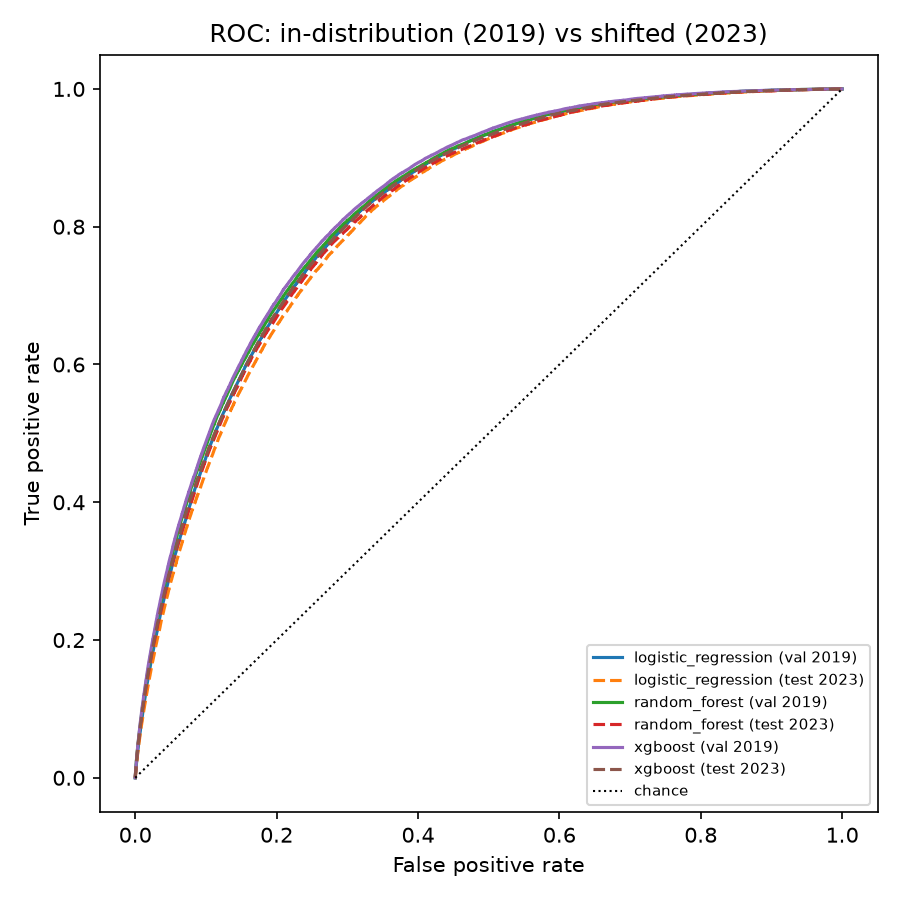
\includegraphics[width=0.75\textwidth]{figures/roc_curves.png}
\caption{ROC curves, in-distribution (2019) vs.\ shifted (2023), all three models.}
\end{figure}

XGBoost is both the strongest performer and the best calibrated out of the box. All three models degrade by roughly the same small amount ($\sim$0.01 AUROC) over six years; for XGBoost this degradation is 0.0081 [95\% CI 0.0057, 0.0103]---small in magnitude, but the interval excludes zero, so it is a real effect at this sample size, not noise. Split conformal prediction targeted 90\% coverage and achieved 89.7\% on the shifted 2023 test set, a drop of 0.0034 [0.0022, 0.0047]---likewise small but real. Failure-detection AUROC is 0.815 [0.814, 0.817]: restricting to the most-confident 20\% of 2023 predictions yields under 1\% error (Figure~\ref{fig:risk-coverage}), meaning the model's confidence remains informative even under shift.

\begin{figure}[h]
\centering
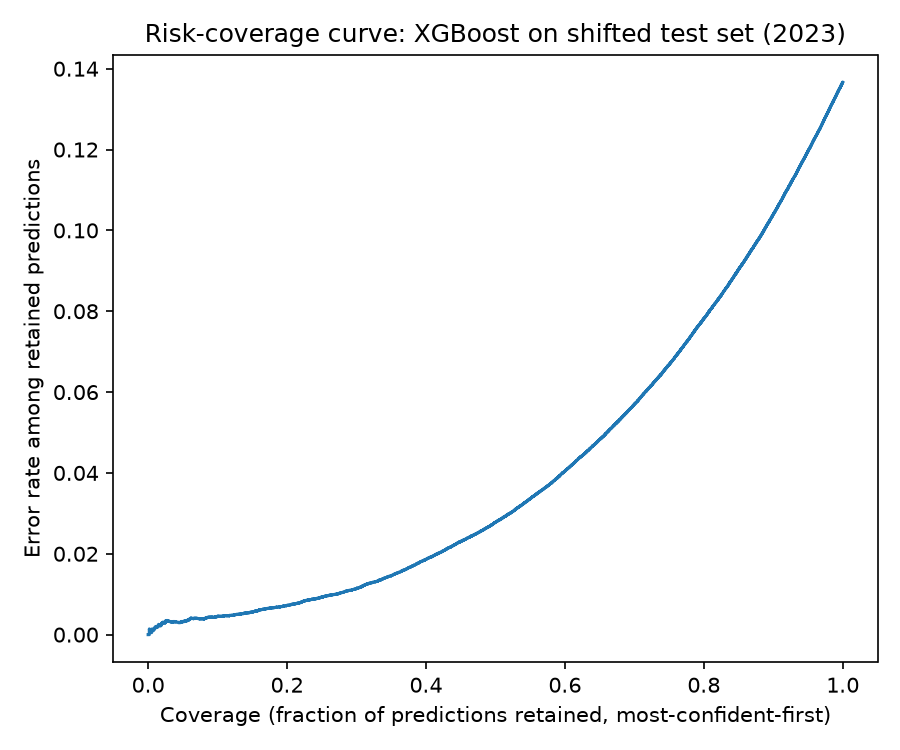
\includegraphics[width=0.6\textwidth]{figures/risk_coverage_curve.png}
\caption{Risk--coverage curve, XGBoost on the shifted 2023 test set.}
\label{fig:risk-coverage}
\end{figure}

\begin{figure}[h]
\centering
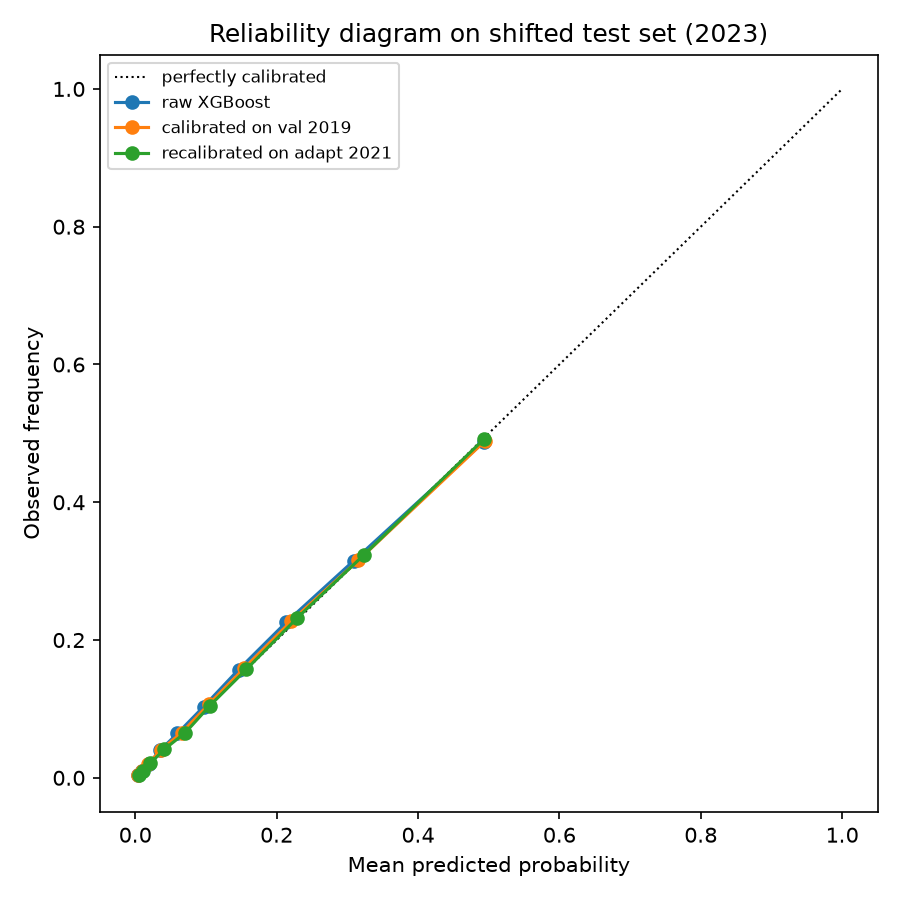
\includegraphics[width=0.6\textwidth]{figures/reliability_diagram.png}
\caption{Reliability diagram: raw, calibrated, and recalibrated XGBoost on the 2023 test set.}
\end{figure}

Recalibrating on a small 2021 sample tightens calibration further (ECE 0.0054 $\to$ 0.0011) with no cost to discrimination (AUROC 0.8276 $\to$ 0.8275)---the expected behavior, since recalibration reshapes probabilities without changing prediction ranking.

\subsection{Subgroup Fairness Under Shift}
\label{sec:subgroup}

\begin{figure}[h]
\centering
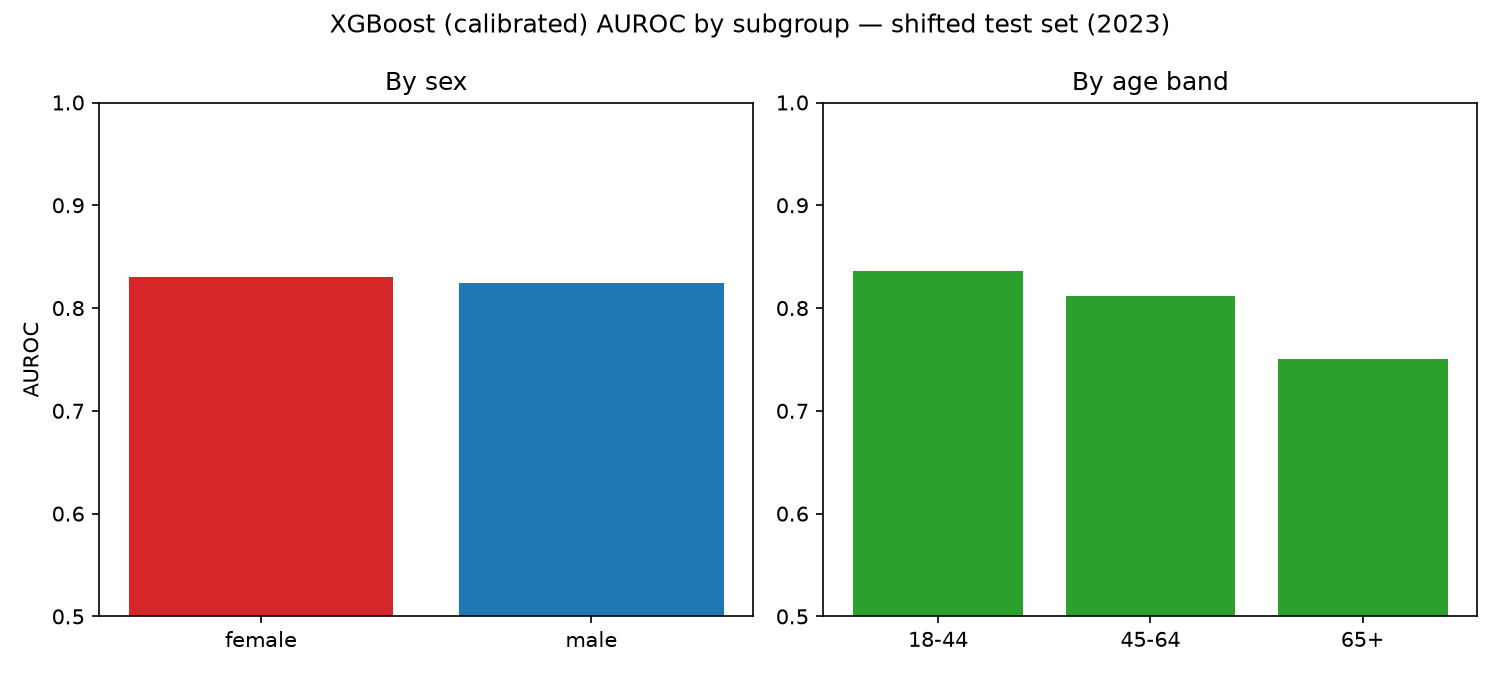
\includegraphics[width=0.75\textwidth]{figures/subgroup_auroc.png}
\caption{XGBoost (calibrated) AUROC by subgroup, shifted test set (2023).}
\end{figure}

Broken out by subgroup on the 2023 test set, sex shows almost no gap (AUROC 0.830 female vs.\ 0.824 male; equalized-odds difference 0.005), but age band shows a substantial one: AUROC falls from 0.836 [95\% CI 0.830, 0.842] (18--44) to 0.811 [0.808, 0.814] (45--64) to \textbf{0.750} [0.748, 0.753] (65+)---a gap between the youngest and oldest bands of 0.0852 [0.0775, 0.0922], clearly excluding zero, and an equalized-odds difference of 0.138, roughly 27x the sex gap. The aggregate temporal result in Section~\ref{sec:temporal} does not surface this at all.

\subsection{Geographic Distribution Shift}
\label{sec:geographic}

\begin{table}[h]
\centering
\begin{tabular}{lccc}
\toprule
Region & AUROC & ECE (cal.\ on NE) & Conformal coverage (target 90\%) \\
\midrule
Northeast (in-region) & 0.827 & 0.000 & 90.0\% \\
Midwest & 0.819 & 0.007 & 88.6\% \\
South & 0.816 & \textbf{0.018} & \textbf{87.3\%} \\
West & 0.827 & 0.004 & 90.2\% \\
\bottomrule
\end{tabular}
\caption{XGBoost trained on Northeast (2023), evaluated by region.}
\end{table}

\begin{figure}[h]
\centering
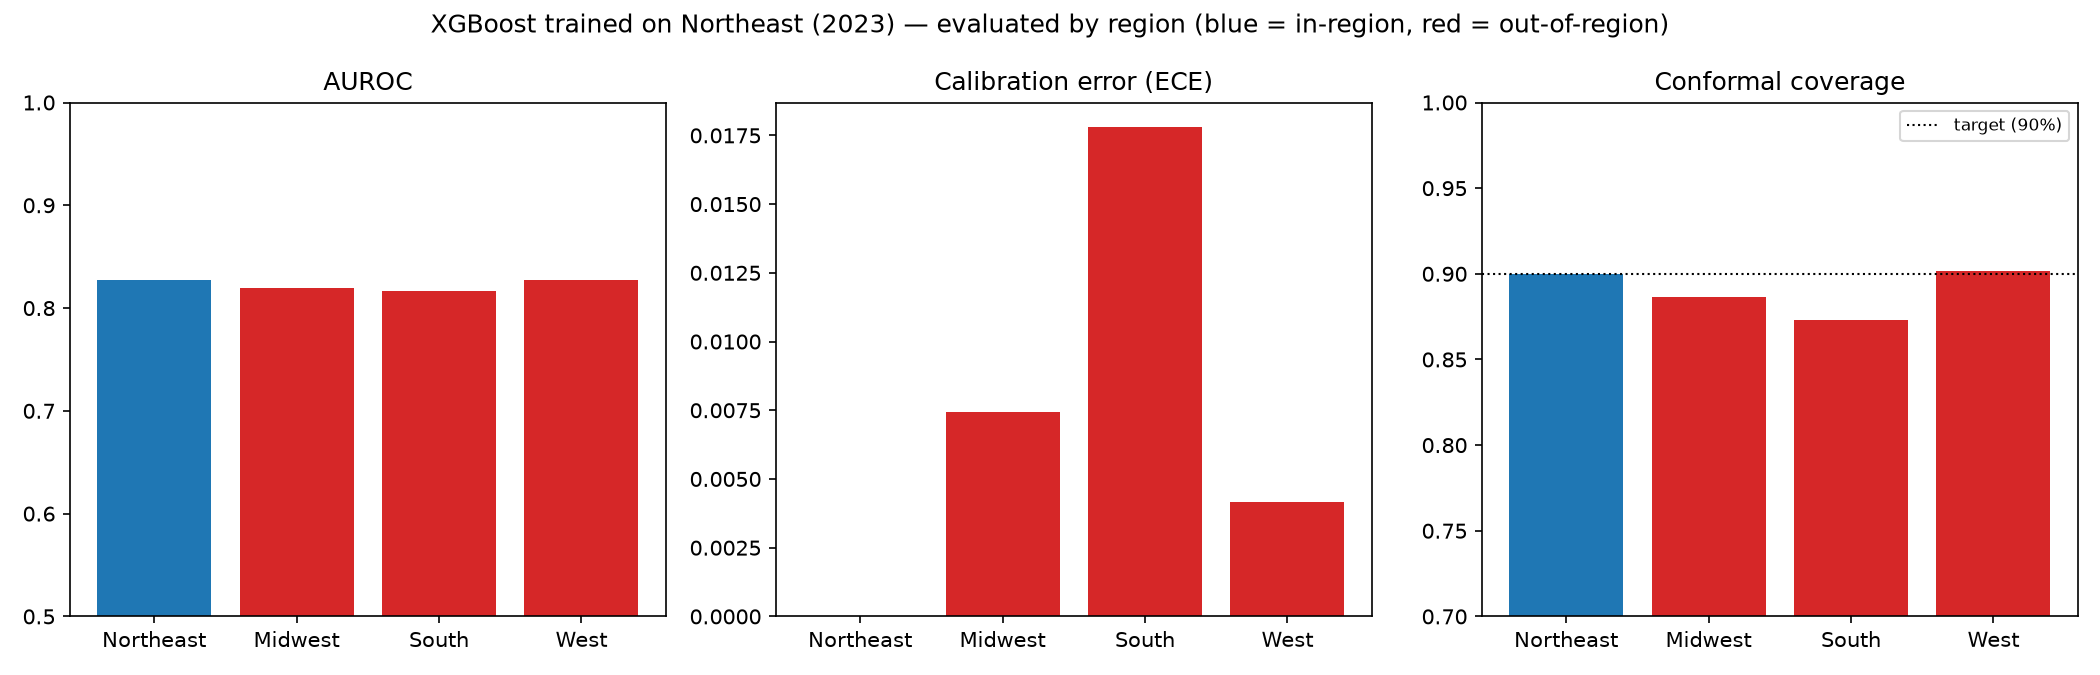
\includegraphics[width=0.85\textwidth]{figures/geographic_shift.png}
\caption{XGBoost trained on Northeast (2023), evaluated by region.}
\end{figure}

Raw discrimination barely moves in absolute terms, echoing Section~\ref{sec:temporal}---though the Northeast-vs-South AUROC gap of 0.0111 [95\% CI 0.0021, 0.0204] does exclude zero, so even this small a difference is statistically real, not sampling noise. Calibration and conformal coverage tell the more consequential story: the South's conformal coverage drop (90.0\% [0.8955, 0.9039] $\to$ 87.3\% [0.8707, 0.8747], 2.7 points) is roughly 9x the drop under the full 6-year temporal shift, and its calibration error is nearly 18x worse than in-region. This aligns with an independently documented pattern---the Southern US has substantially higher diabetes prevalence than the Northeast (16.9\% vs.\ $\sim$12.3\% in this data, consistent with the CDC's ``diabetes belt'')---so a model calibrated on the Northeast's lower base rate is systematically overconfident when applied to the South's higher one. Failure-detection AUROC still holds up reasonably everywhere (0.80--0.82).

\subsection{Weighted Conformal Prediction}
\label{sec:weighted-conformal}

\begin{table}[h]
\centering
\begin{tabular}{lccc}
\toprule
Region & Unweighted coverage & Weighted coverage & Mean set size (unw.\ $\to$ w.) \\
\midrule
Midwest & 88.6\% & \textbf{89.6\%} & 1.06 $\to$ 1.09 \\
South & 87.3\% & \textbf{88.7\%} & 1.07 $\to$ 1.11 \\
West & 90.2\% & 90.0\% & 1.05 $\to$ 1.04 \\
\bottomrule
\end{tabular}
\caption{Conformal coverage, unweighted vs.\ weighted, by region.}
\end{table}

\begin{figure}[h]
\centering
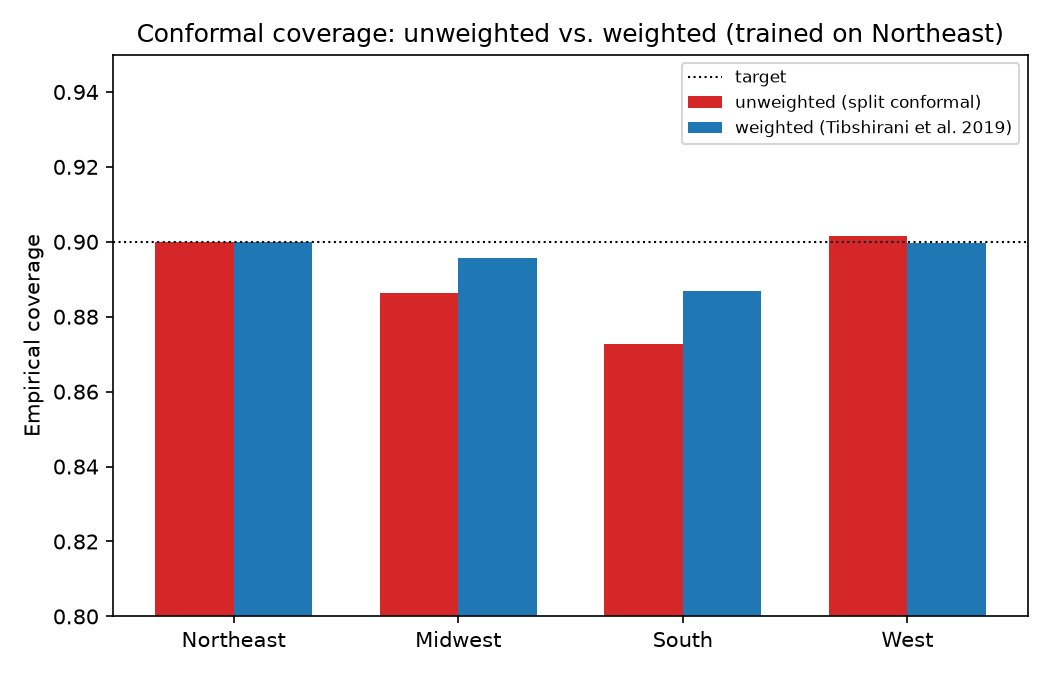
\includegraphics[width=0.7\textwidth]{figures/weighted_conformal.png}
\caption{Conformal coverage, unweighted vs.\ weighted, by region.}
\end{figure}

Weighting closes roughly half the South's coverage gap (+0.0142 [95\% CI 0.0135, 0.0148]) and nearly all of the Midwest's (+0.0094 [0.0088, 0.0099]), at the cost of modestly larger prediction sets---the expected trade-off, and in both cases the improvement is clearly real, not noise. For the West, where there was barely any gap to begin with, the bootstrap CI reveals something more precise than ``no effect'': weighting produces a small but statistically significant \emph{decrease} in coverage, $-0.0021$ [$-0.0024$, $-0.0018$]. That interval excludes zero, so it isn't sampling noise either---reweighting has a genuine, if small, cost even where there is little real shift to correct for. That's a more honest characterization than ``no effect,'' and a useful practical caveat: weighted conformal prediction is not a free action to apply by default, it is a trade specifically worth making where the coverage gap is large enough to be worth the (small) risk of making things marginally worse where it isn't. It does not fully close the South's gap either way: the density-ratio estimate is only as good as the domain classifier estimating it, and this particular covariate shift is large.

\subsection{Deep Ensembles and MC-Dropout}
\label{sec:deep-ensemble}

\begin{table}[h]
\centering
\resizebox{\textwidth}{!}{%
\begin{tabular}{lccc}
\toprule
Model & AUROC (test 2023) & ECE, raw (test 2023) & Failure-detection AUROC \\
\midrule
Deep ensemble (10 members) & 0.827 & 0.0099 & 0.800 (disagreement) \\
MC-dropout (single net) & --- & --- & 0.786 \\
XGBoost (raw / calibrated) & 0.828 & 0.0054 & 0.815 (calibrated) \\
\bottomrule
\end{tabular}%
}
\caption{Deep ensemble / MC-dropout (AMD MI300X) vs.\ XGBoost, test 2023.}
\end{table}

\begin{figure}[h]
\centering
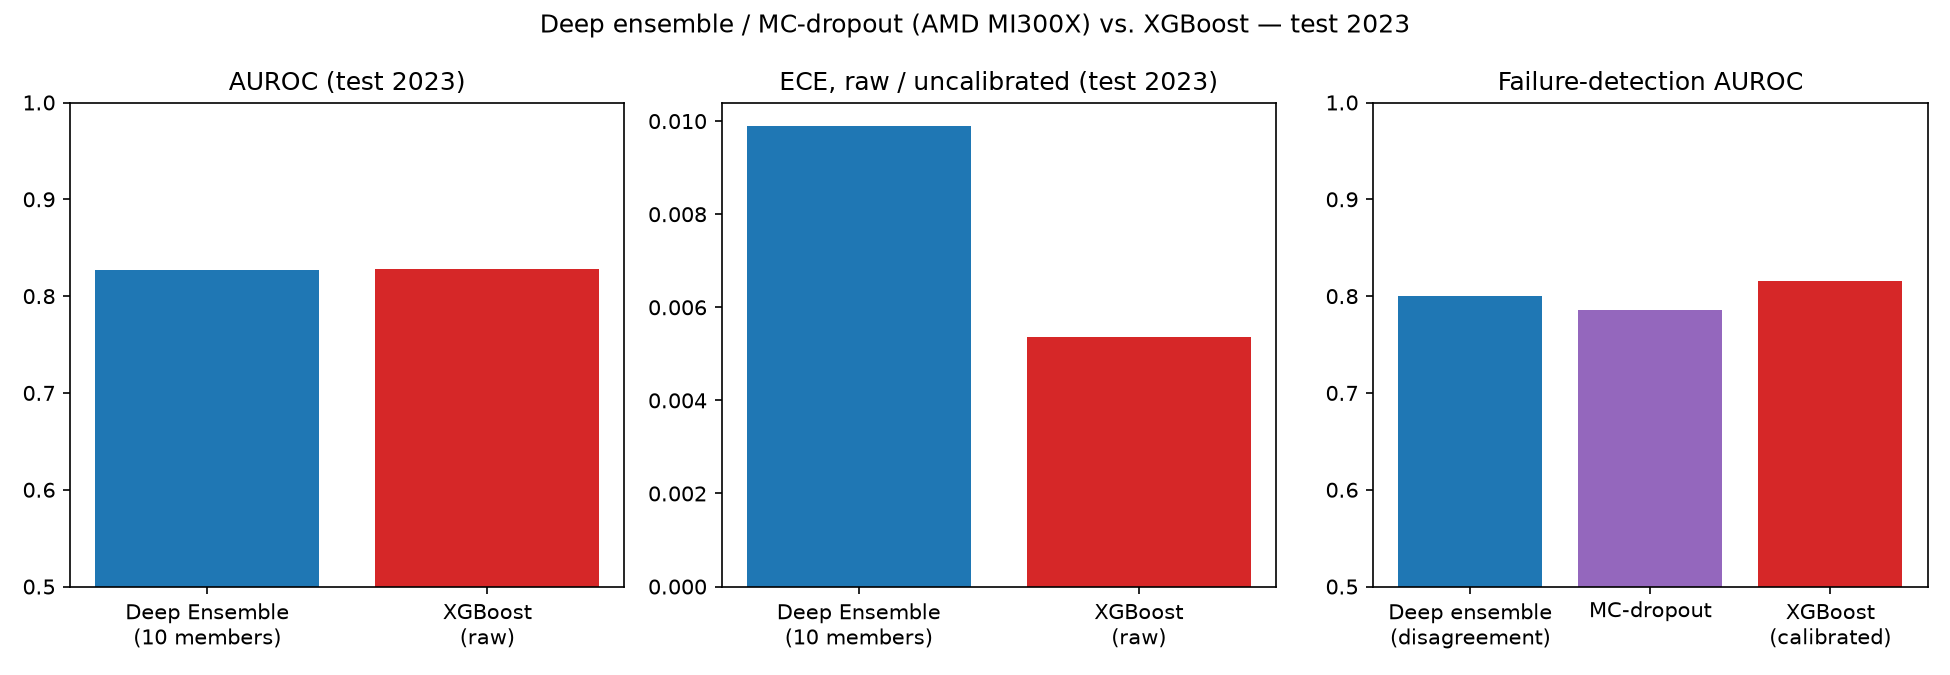
\includegraphics[width=0.9\textwidth]{figures/deep_ensemble_comparison.png}
\caption{Deep ensemble / MC-dropout (AMD MI300X) vs.\ XGBoost, test 2023.}
\end{figure}

Trained on an AMD Instinct MI300X (10 members, 50 epochs each), the deep ensemble matches XGBoost's discrimination almost exactly: AUROC 0.8272 [95\% CI 0.8254, 0.8286] vs.\ XGBoost's 0.8275, a paired gap of just $-0.0003$ [$-0.0006$, $-0.0001$]. That interval excludes zero---with 418{,}492 test rows the difference is technically detectable---but a gap this small is practically a tie, and it's a tie despite the ensemble using none of gradient boosting's tree-structure inductive bias. Its raw calibration is worse than XGBoost's raw calibration (ECE 0.0098 [0.0090, 0.0108] vs.\ 0.0054), consistent with \citet{ovadia2019trust}'s finding that ensembles are reasonably but not perfectly calibrated out of the box. Ensemble disagreement---the variance across members' predictions---is a genuinely useful uncertainty signal (failure-detection AUROC 0.8001 [0.7985, 0.8017]), and outperforms MC-dropout on the same trained network (0.7862 [0.7844, 0.7881]) by 0.0139 [0.0129, 0.0149]---non-overlapping intervals, so this isn't a close call, consistent with the literature's general finding that ensembles give better-behaved uncertainty than dropout-based approximation alone. Both remain informative, in the same range as XGBoost's calibrated signal (0.815) from Section~\ref{sec:temporal}---the finding that uncertainty survives this shift is not specific to gradient-boosted trees, and this is now shown with the same statistical rigor as every other result in the paper.

\section{Discussion}

The central pattern across Sections~\ref{sec:temporal}--\ref{sec:weighted-conformal} is that \textbf{shift magnitude, not merely shift's presence, determines how much of the reliability story holds}---and that this magnitude varies enormously depending on which dimension of shift is measured and at what level of aggregation. The temporal shift, averaged over the whole population, looked mild. It wasn't mild for the 65+ subgroup, and it wasn't mild when geography rather than time was the shift axis: the South's conformal coverage came measurably closer to the kind of breakdown the literature predicts \citep{tibshirani2019conformal} than six years of temporal drift ever did. An evaluation that stopped at the aggregate temporal result would have concluded the model was essentially shift-robust. It isn't---not for the 65+ subgroup, and not for the South.

This has a direct methodological implication for how uncertainty-aware systems should be evaluated before deployment: a single shift axis, measured only in aggregate, is not sufficient evidence of reliability. The subgroup and geographic analyses here were comparatively cheap to run once the core pipeline existed---the marginal cost of checking multiple shift dimensions is small relative to the risk of missing the one that matters.

The weighted conformal result (Section~\ref{sec:weighted-conformal}) is encouraging but incomplete in a specific, informative way: it demonstrates that the theoretically-correct response to detected covariate shift genuinely helps, while also demonstrating its limit---a simple domain classifier cannot fully correct for a shift this large from so few calibration examples. That gap is itself worth reporting, rather than papering over with a stronger domain classifier tuned to close it; a more expressive density-ratio estimator is a natural next step, but the honest finding at this stage is partial, not complete, recovery. The bootstrap CI on the West result sharpens this further: reweighting is not a free safeguard to apply indiscriminately, since it produced a small but statistically significant coverage \emph{cost} precisely where there was little shift to correct for. The practical implication is to apply it selectively---where a shift has actually been detected---rather than by default.

The deep ensemble comparison (Section~\ref{sec:deep-ensemble}) adds one more piece to this picture: uncertainty surviving distribution shift is not an artifact specific to gradient-boosted trees. A neural network ensemble with no tree-structure inductive bias reaches statistically the same discrimination ceiling as XGBoost (a paired gap of $-0.0003$, technically significant only because of the sample size, practically a tie) and produces a comparably informative uncertainty signal via member disagreement, even though its raw calibration is worse out of the box. That the central finding replicates across two structurally different model families is modest additional evidence that it reflects something about the \emph{data and shift}, rather than an idiosyncrasy of one algorithm---and with this section's bootstrap CIs now in place, every result in the paper is held to the same statistical standard, not just the classical baselines.

\section{Limitations}

\begin{itemize}[leftmargin=*]
\item Single train year (2017) rather than a multi-year training window, chosen to keep the pre/post-shift boundary clean.
\item Missing values handled via median imputation fit on the training split only; missingness rates are modest ($<$13\% for every feature).
\item The feature set omits fruit/vegetable intake and income due to within-window definitional changes, making it narrower than the ``Diabetes Health Indicators''-style feature sets used elsewhere in the literature.
\item The geographic-shift domain classifier (Sections~\ref{sec:geographic}--\ref{sec:weighted-conformal}) is a plain logistic regression on the same 15 features; a more expressive estimator might close more of the coverage gap.
\item This is a methodological study of reliability under shift, not a clinical validation---health-risk prediction is the application domain, not a deployment claim.
\end{itemize}

\section{Conclusion}

Uncertainty-aware evaluation of a real diabetes-risk model under real distribution shift shows that calibration and conformal coverage are far more sensitive to shift magnitude than raw discrimination is, that this sensitivity is easy to miss when only one shift dimension or only the aggregate is examined, and that a theoretically-motivated fix for detected coverage loss (weighted conformal prediction) works, partially. The practical recommendation this supports is straightforward: evaluate uncertainty-aware systems across multiple, independent shift dimensions---not just time---before treating aggregate stability as evidence of reliability.

\section*{Acknowledgments}

This research is conducted with mentorship from Avneh Singh Bhatia at Exea Labs, who arranged access to an AMD Instinct MI300X accelerator, provided by AMD, for the deep-learning experiments in Section~\ref{sec:deep-ensemble}.

That access mattered in a specific, honest way. This paper's neural-network baseline (a 10-member deep ensemble and MC-dropout network, 50 epochs each) is small by modern deep-learning standards, but it is precisely the experiment that a CPU-only research setup would have left as a reduced-scale correctness check rather than a full, paper-ready result---Section~\ref{sec:deep-ensemble} would still read ``pending'' without it. The MI300X's compute made the full-scale run take minutes rather than hours, and the pre-configured ROCm/PyTorch environment meant the entire pipeline---clone, install, download data, train, evaluate---ran end-to-end within a single short session with no framework friction. The practical result: the paper's central finding, that uncertainty survives distribution shift, could be tested on a second, structurally different model family (Section~\ref{sec:deep-ensemble}) rather than resting on gradient-boosted trees alone. Our thanks to AMD and Exea Labs for making that possible.

\bibliographystyle{plainnat}
\bibliography{references}

\end{document}
